
\documentclass[a4paper,11pt]{article}
\usepackage[a4paper, margin=8em]{geometry}

% usa i pacchetti per la scrittura in italiano
\usepackage[french,italian]{babel}
\usepackage[T1]{fontenc}
\usepackage[utf8]{inputenc}
\frenchspacing 

% usa i pacchetti per la formattazione matematica
\usepackage{amsmath, amssymb, amsthm, amsfonts}

% usa altri pacchetti
\usepackage{gensymb}
\usepackage{hyperref}
\usepackage{standalone}

% imposta il titolo
\title{Appunti Elettronica Digitale}
\author{Luca Seggiani}
\date{2026}

% imposta lo stile
% usa helvetica
\usepackage[scaled]{helvet}
% usa palatino
\usepackage{palatino}
% usa un font monospazio guardabile
\usepackage{lmodern}

\renewcommand{\rmdefault}{ppl}
\renewcommand{\sfdefault}{phv}
\renewcommand{\ttdefault}{lmtt}

% disponi il titolo
\makeatletter
\renewcommand{\maketitle} {
	\begin{center} 
		\begin{minipage}[t]{.8\textwidth}
			\textsf{\huge\bfseries \@title} 
		\end{minipage}%
		\begin{minipage}[t]{.2\textwidth}
			\raggedleft \vspace{-1.65em}
			\textsf{\small \@author} \vfill
			\textsf{\small \@date}
		\end{minipage}
		\par
	\end{center}

	\thispagestyle{empty}
	\pagestyle{fancy}
}
\makeatother

% disponi teoremi
\usepackage{tcolorbox}
\newtcolorbox[auto counter, number within=section]{theorem}[2][]{%
	colback=blue!10, 
	colframe=blue!40!black, 
	sharp corners=northwest,
	fonttitle=\sffamily\bfseries, 
	title=~\thetcbcounter: #2, 
	#1
}

% disponi definizioni
\newtcolorbox[auto counter, number within=section]{definition}[2][]{%
	colback=red!10,
	colframe=red!40!black,
	sharp corners=northwest,
	fonttitle=\sffamily\bfseries,
	title=~\thetcbcounter: #2,
	#1
}

% U.D.M
\newcommand{\amp}{\ensuremath{\mathrm{A}}}
\newcommand{\volt}{\ensuremath{\mathrm{V}}}
\newcommand{\meter}{\ensuremath{\mathrm{m}}}
\newcommand{\second}{\ensuremath{\mathrm{s}}}
\newcommand{\farad}{\ensuremath{\mathrm{F}}}
\newcommand{\henry}{\ensuremath{\mathrm{H}}}
\newcommand{\siemens}{\ensuremath{\mathrm{S}}}

% circuiti
\usepackage{circuitikz}
\usetikzlibrary{babel}

% disegni
\usepackage{pgfplots}
\pgfplotsset{width=10cm,compat=1.9}

% disponi codice
\usepackage{listings}
\usepackage[table]{xcolor}

\definecolor{codegreen}{rgb}{0,0.6,0}
\definecolor{codegray}{rgb}{0.5,0.5,0.5}
\definecolor{codepurple}{rgb}{0.58,0,0.82}
\definecolor{backcolour}{rgb}{0.95,0.95,0.92}

\lstdefinestyle{codestyle}{
		backgroundcolor=\color{black!5}, 
		commentstyle=\color{codegreen},
		keywordstyle=\bfseries\color{magenta},
		numberstyle=\sffamily\tiny\color{black!60},
		stringstyle=\color{green!50!black},
		basicstyle=\ttfamily\footnotesize,
		breakatwhitespace=false,         
		breaklines=true,                 
		captionpos=b,                    
		keepspaces=true,                 
		numbers=left,                    
		numbersep=5pt,                  
		showspaces=false,                
		showstringspaces=false,
		showtabs=false,                  
		tabsize=2
}

\lstdefinestyle{shellstyle}{
		backgroundcolor=\color{black!5}, 
		basicstyle=\ttfamily\footnotesize\color{black}, 
		commentstyle=\color{black}, 
		keywordstyle=\color{black},
		numberstyle=\color{black!5},
		stringstyle=\color{black}, 
		showspaces=false,
		showstringspaces=false, 
		showtabs=false, 
		tabsize=2, 
		numbers=none, 
		breaklines=true
}

\lstdefinelanguage{javascript}{
	keywords={typeof, new, true, false, catch, function, return, null, catch, switch, var, if, in, while, do, else, case, break},
	keywordstyle=\color{blue}\bfseries,
	ndkeywords={class, export, boolean, throw, implements, import, this},
	ndkeywordstyle=\color{darkgray}\bfseries,
	identifierstyle=\color{black},
	sensitive=false,
	comment=[l]{//},
	morecomment=[s]{/*}{*/},
	commentstyle=\color{purple}\ttfamily,
	stringstyle=\color{red}\ttfamily,
	morestring=[b]',
	morestring=[b]"
}

% disponi sezioni
\usepackage{titlesec}

\titleformat{\section}
	{\sffamily\Large\bfseries} 
	{\thesection}{1em}{} 
\titleformat{\subsection}
	{\sffamily\large\bfseries}   
	{\thesubsection}{1em}{} 
\titleformat{\subsubsection}
	{\sffamily\normalsize\bfseries} 
	{\thesubsubsection}{1em}{}

% disponi alberi
\usepackage{forest}

\forestset{
	rectstyle/.style={
		for tree={rectangle,draw,font=\large\sffamily}
	},
	roundstyle/.style={
		for tree={circle,draw,font=\large}
	}
}

% disponi algoritmi
\usepackage{algorithm}
\usepackage{algorithmic}
\makeatletter
\renewcommand{\ALG@name}{Algoritmo}
\makeatother

% disponi numeri di pagina
\usepackage{fancyhdr}
\fancyhf{} 
\fancyfoot[L]{\sffamily{\thepage}}

\makeatletter
\fancyhead[L]{\raisebox{1ex}[0pt][0pt]{\sffamily{\@title \ \@date}}} 
\fancyhead[R]{\raisebox{1ex}[0pt][0pt]{\sffamily{\@author}}}
\makeatother

\begin{document}
% sezione (data)
\section{Lezione del 27-03-26}

% stili pagina
\thispagestyle{empty}
\pagestyle{fancy}

% testo
Nella scorsa lezione abbiamo introdotto i transistori \textbf{BJT} (\textit{Bipolar Junction Transistor}). Iniziamo adesso a vedere come risolvere circuiti che contengono tali componenti.

\subsubsection{Risoluzione di circuiti con BJT}
Avremo a disposizione diversi metodi di risoluzione per determinare la risposta del transistore ai \textit{grandi segnali} (come avevamo per il diodo a 6.1.3). Innanzitutto, ai grandi segnali significa determinare il punto di riposo, cioè le grandezze:
$$
V_{BEQ}, \ I_{BQ} \ V_{CEQ} \ I_{CQ}
$$
cioè tensioni e correnti di base e di collettore in condizioni di equilibrio.

I metodi che avremo saranno quindi:
\begin{itemize}
	\item Metodi \textit{analitici}: basati sul modello di Ebers-Moll o eventuali modelli semplificati derivanti da questo;
	\item Metodi \textit{grafici}: consistono nella tracciatura della retta di carico (vista sempre in 6.1.3) sulle caratteristiche di ingresso e di uscita del BJT (viste nella scorsa lezione, legano le correnti di base e di collettore alle relative tensioni).
\end{itemize}

Vediamo ad esempio il seguente circuito:
\begin{center}
\begin{circuitikz}
	% NPN

	\draw (0,2) to[ american voltage source, l_=$v_{BB}$] (0,0);
	\draw (0,2) to[ resistor, l=$R_B$] (2,2) to[ short, i=$i_B$] (4,2);
	\draw (0,0) -- (8,0);
	\draw (8,2) to[ american voltage source, l=$v_{CC}$] (8,0);
	\draw (4.5,1.5) -- (4.5, 0);
	\draw (8,2) to[ resistor, l_=$R_C$] (8,4)
		to[ short, i=$i_C$] (4.5, 4) -- (4.5,2.5);

	\node[npn] at(4.5,2) {};

	\node at(5,3.75) {$+$};
	\node at(5,2) {$v_{CE}$};
	\node at(5,0.25) {$-$};
	
	\node at(3.5,1.75) {$+$};
	\node at(3.5,1) {$v_{BE}$};
	\node at(3.5,0.25) {$-$};

	\node at(4.8, 2.4) {$\scriptstyle C$};
	\node at(3.8, 2.2) {$\scriptstyle B$};
	\node at(4.8, 1.6) {$\scriptstyle E$};
\end{circuitikz}
\end{center}
già introdotto alla scorsa lezione per la discussione delle caratteristiche di ingresso e di uscita ad emettitore comune.

Possiamo quindi impostare le equazioni alle maglie:
\[
	\begin{cases}
		V_{BB} = R_B I_B + V_{BE} \\
		V_{CC} = R_C I_C + V_{CE}
	\end{cases}
\]
e le caratteristiche di ingresso e di uscita del BJT:
\[
	\begin{cases}
		I_B = f(V_{BE}, V_{CE}) = I_B I_{ES} e^{\frac{V_{BE}}{V_T}} \\
		I_C = f(I_B, V_{CE}) = \beta_F I_B 
	\end{cases}
\]

\begin{itemize}
\item \textbf{\textsf{Metodo grafico}} \\
Proviamo a risolvere il circuito col metodo grafico. Per fare ciò prenderemo la retta di carico ricavata dall'equazione della maglia su $V_{BB}$, e la tracceremo sul grafico sovrapposta alla curva di risposta in ingresso del BJT.

Quindi, ricavato un valore valido di $I_B$, possiamo selezionare tale valore sul grafico della $I_C$ in funzione di $V_{CE}$ al variare di $I_B$. Sempre per intersezione di grafici, troveremo la corrente $I_C$ di collettore.

\begin{center}
	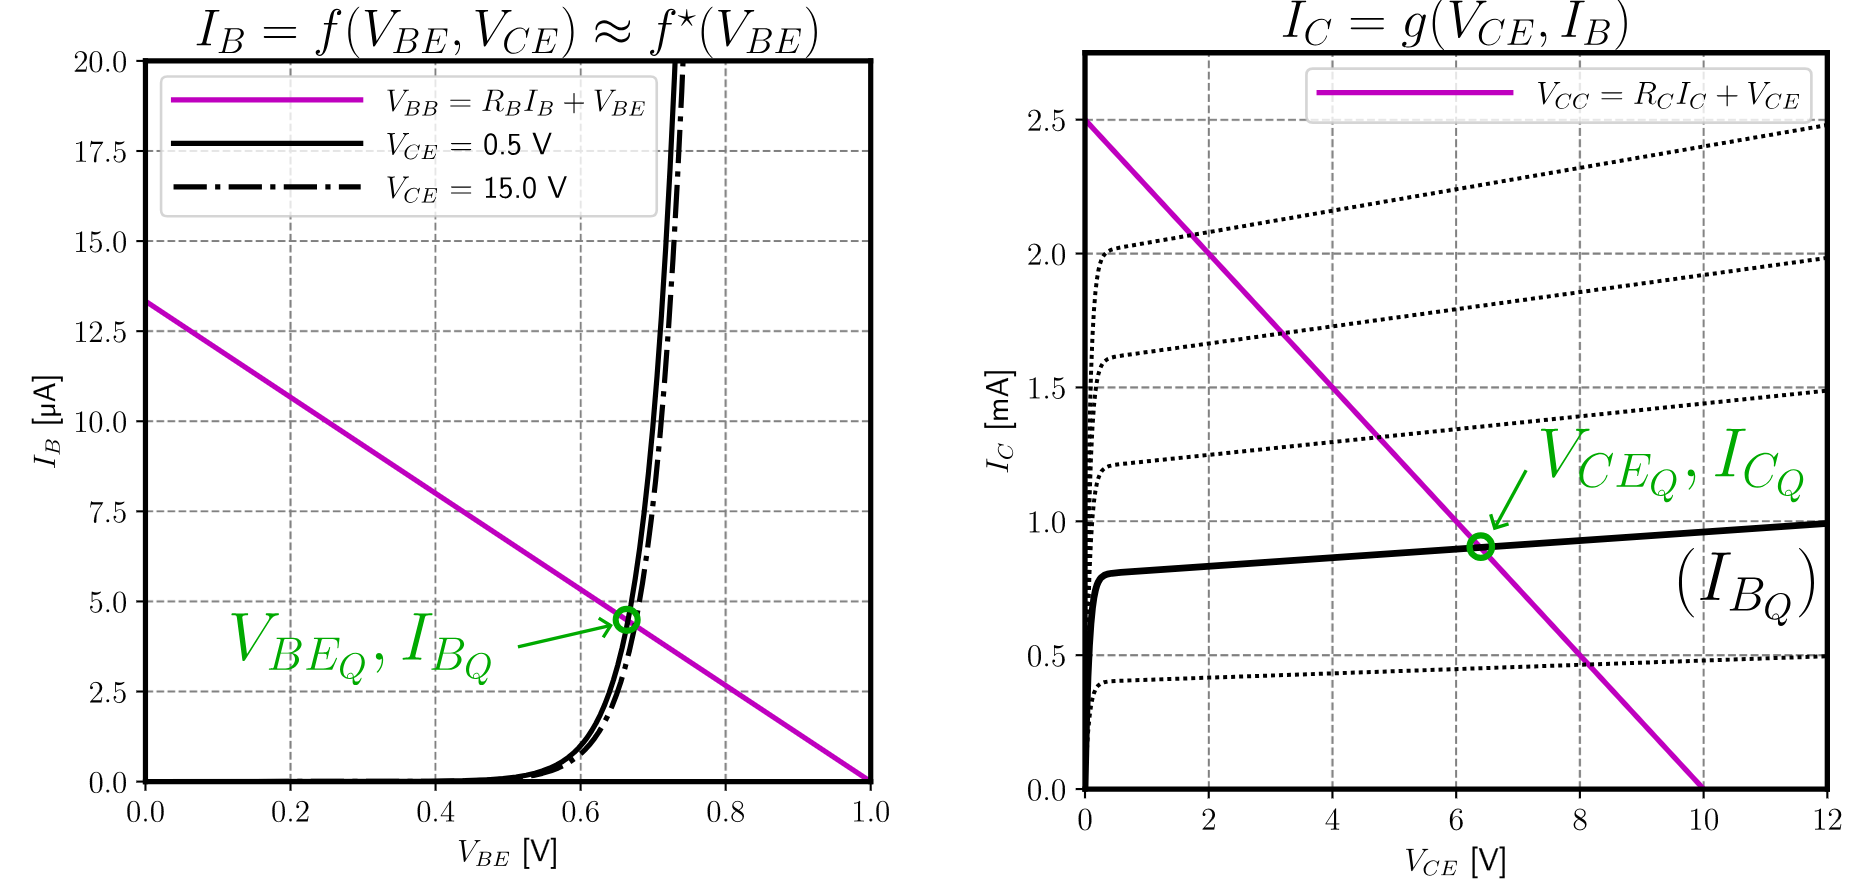
\includegraphics[scale=0.21]{../figures/bjt_graph.png}
\end{center}

Questo metodo ci dà un errore dato dal fatto che, presa la caratteristica di ingresso approssimata:
$$
I_B = f(V_{BE}, V_{CE}) = (1 - \alpha_F) I_{ES} e^{V_{BE}}{T} \\
$$
trascuriamo la $V_{CE}$ per il calcolo di $I_B$ (effetto di Early trascurabile). Questo ci è spesso possibile in quanto la differenza effettiva fra i valori che otteniamo è minima (dal grafico si vede la minima differenza variando $V_{CE}$ da $0.5 \, \mathrm{V}$ a $15 \, \mathrm{V}$);

\item \textbf{\textsf{Metodo analitico}} \\
Per il metodo analitico, assumiamo di trovarci in ZAD e prendiamo il modello di Ebers-Moll semplificato:
$$
I_{BQ} = (1 - \alpha_F) I_{ES} e^{\frac{V_{BEQ}}{V_T}}
$$
in tal caso l'effetto di Early all'ingresso è automaticamente trascurato (il modello di Ebers-Moll non lo considera a priori). Possiamo quindi sostituire questa nell'equazione della retta di carico, per ottenere:
$$
V_{BB} = R_B (1 - \alpha_F) I_{ES}e^{\frac{V_{BEQ}}{V_T}} + V_{BEQ}
$$
Notiamo però che questa è un'equazione trascendente con incognita $V_{BEQ}$, di difficile risoluzione analitica. Il meglio che possiamo fare è trovare una soluzione approssimata per via numerica (a mano o sfruttando un calcolatore);

\item \textbf{\textsf{Metodo analitico semplificato}} \\
Prendiamo quindi un modello a caduta costante della giunzione BE (assunto il BJT in ZAD). Questo sarà esattamente uguale al modello a caduta costante del diodo preso in 6.1.3, con:
$$
V_{BEQ} = V_\gamma = 0.7 \, \mathrm{V}
$$

Sostituendo ciò nell'equazione della retta di carico (cioè semplicemente risolvendo la maglia), si ottiene:
$$
I_{BQ} = \frac{V_{BB} - V_\gamma}{R_B}
$$
cioè siamo riusciti a semplificare di molto (approssimando) un'equazione trascendente con incognita $V_{BEQ}$, rendendola qualcosa che siamo effettivamente capaci di risolvere.

A questo punto l'effetto Early viene trascurato anche sulla caratteristica di uscita, quindi si usa quindi la semplice relazione:
$$
I_{CQ} = \beta_F I_{BQ}
$$

La $V_{CEQ}$ si avrà sempre dalle equazioni di maglia:
$$
V_{CEQ} = V_{CC} - R_C \beta_F I_{BQ}
$$
verificando che $V_{CEQ} > V_{CE, \, \mathrm{sat}} \approx 0.2 \, \mathrm{V}$.

Avremo quindi trovato, in maniera approssimata, tutte le condizioni a riposo, cioè le grandezze:
$$
V_{BEQ}, \ I_{BQ} \ V_{CEQ} \ I_{CQ}
$$

\item \textbf{\textsf{Metodo analitico semplificato generale}}

Estendiamo quindi il metodo di risoluzione alle regioni di saturazione e interdizione (oltre la ZAD), mostrando anche le condizioni da verificare, nel seguente schema:
\begin{center}
	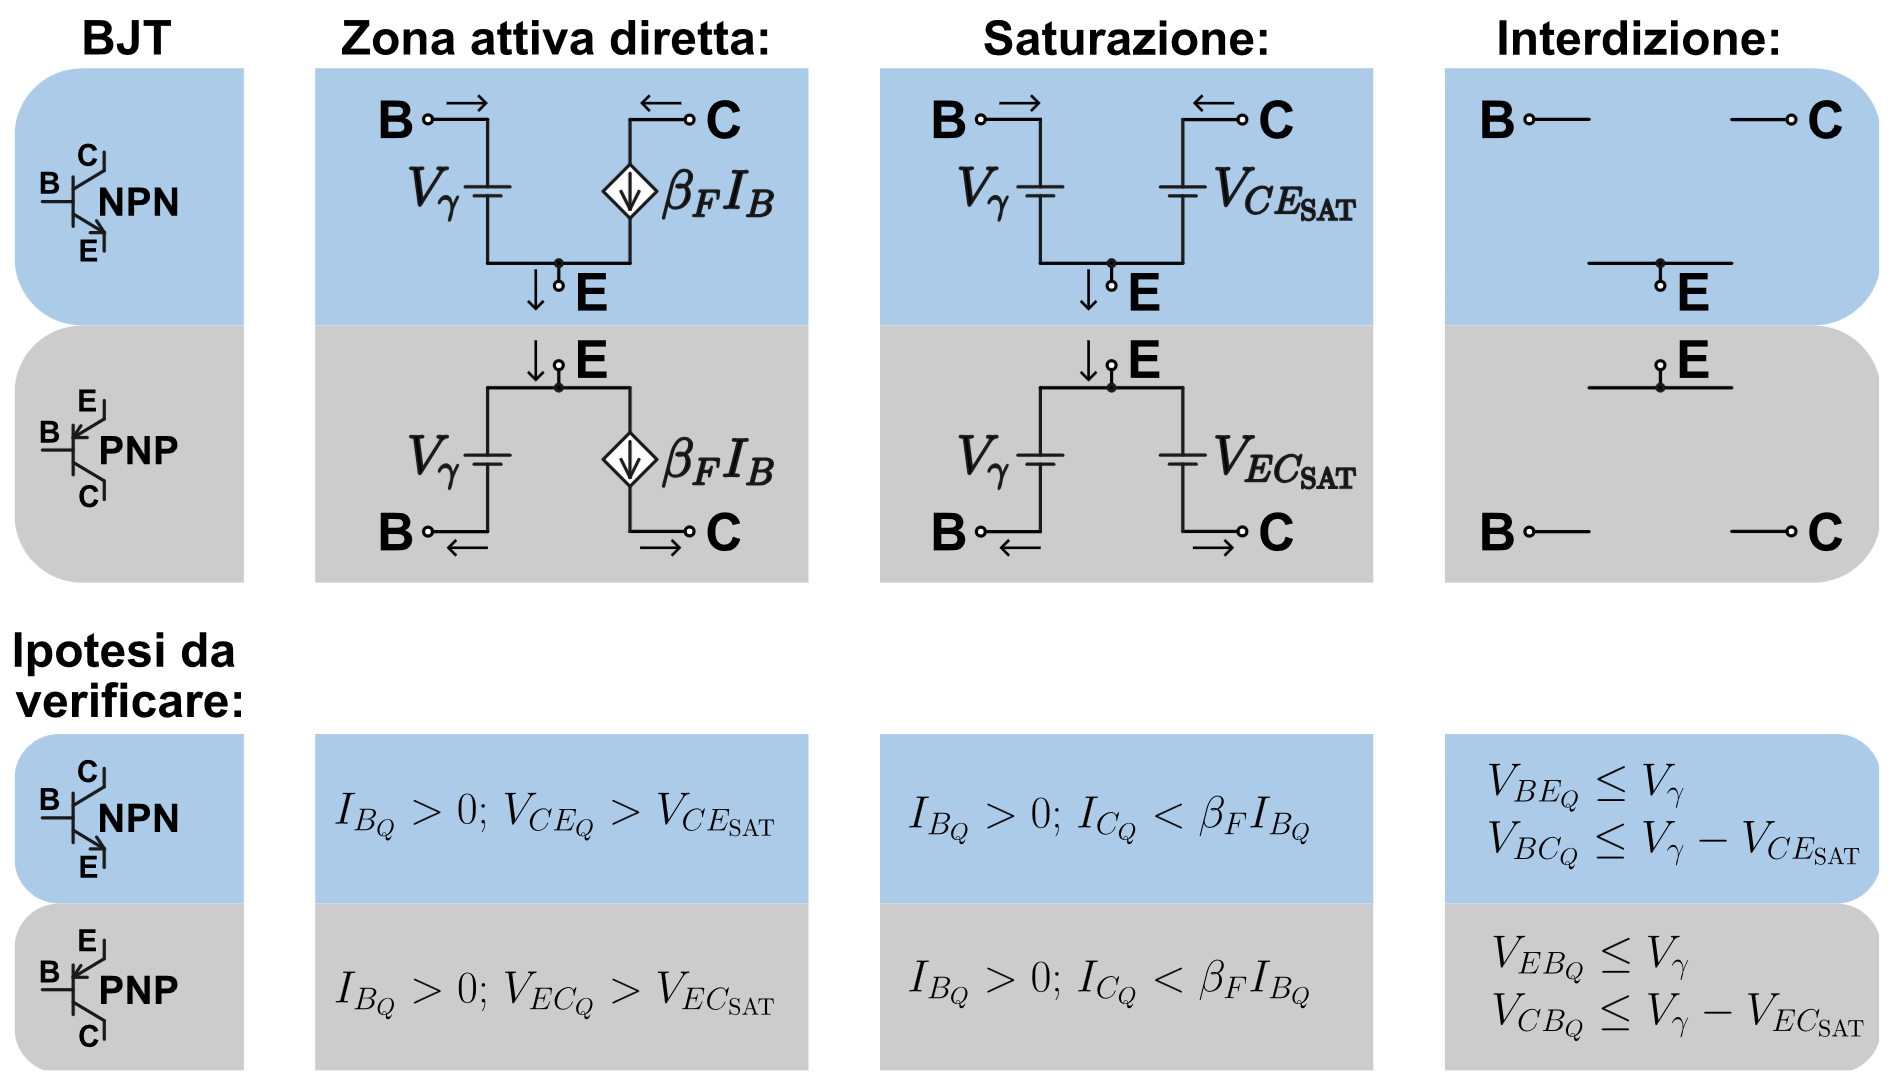
\includegraphics[scale=0.2]{../figures/bjt_resolv.png}
\end{center}

Discutiamo lo schema:
\begin{itemize}
	\item \textbf{\textsf{Zona Attiva Diretta}} \\
		Questo è il modello che abiamo discusso finora, dove assumiamo la caduta fra base ed emettitore come costante (pari a $V_\gamma \approx 0.7 \, \mathrm{V}$), e usiamo la semplice approssimazione lineare $I_C = \beta_F I_B$ per la corrente al collettore. La situazione al PNP è la stessa ma invertendo collettore ed emettitore.

		Notiamo che in questo caso dobbiamo verificare che la corrente alla base sia maggiore di 0 (cioè siamo in transistore aperto), ovvero $I_{BQ} > 0$, e che la tensione collettore-emettitore sia maggiore di quella di saturazione, ovvero $V_{CEQ} > V_{CE \, \mathrm{sat}}$;

	\item \textbf{\textsf{Saturazione}} \\
		In saturazione sostituiamo il generatore di corrente al collettore con una tensione costante pari alla tensione di saturazione (che assumiamo già raggiunta) $V_{CE \, \mathrm{sat}}$.

		In questo caso le condizioni da soddisfare saranno che la corrente alla base sia comunque maggiore di 0, ovvero $I_{BQ} > 0$, e che anche la corrente al collettore sia minore del valore in ZAD, cioè $I_C < \beta_F I_B$;

	\item \textbf{\textsf{Interdizione}} \\
		In interdizione banalmente prendiamo circuiti aperti.

		Qui le condizioni da soddisfare saranno semplicemente che le tensioni a base-emettitore e base-collettore siano:
$$
V_{BEQ} \leq V_\gamma, \quad V_{BCQ} \leq V_\gamma - V_{CE \, \mathrm{sat}}
$$
\end{itemize}

\end{itemize}

\subsection{Analisi di un inverter a carico resistivo}
Vediamo quindi un primo circuito formato da transistor, formato da un singolo transistore NPN:

\begin{center}
\begin{circuitikz}
% Transistor
\draw (0,0) node[npn, anchor=E] (Q1) {};

% Emitter to ground
\draw (Q1.E) -- ++(0,-1) node[ground]{};

% Collector resistor and Vcc
\draw (Q1.C) -- ++(0,1) to[R, l=$R_C$] ++(0,2) node[above]{$V_{CC}$};

% Output node
\draw (Q1.C) -- ++(1,0) node[right]{$V_{out}$};

% Base resistor and input
\draw (Q1.B) -- ++(-1,0) to[R, l=$R_B$] ++(-2,0) node[left]{$V_{in}$};

% Current labels
\draw[->] (Q1.B) ++(-0.3,0.3) -- ++(0.6,0) node[midway, above]{$I_B$};
\draw[->] (Q1.C) ++(0.3,1) -- ++(0,-0.8) node[midway, right]{$I_C$};

\end{circuitikz}
\end{center}

Assumiamo che la tensione di ingresso $V_{in}$ varia da 0 fino al valore $V_{CC}$ (ad esempio, $5 \, \mathrm{V}$) a passi discreti, e che il valore della tensione di uscita viene registrata una volta esauriti i transitori. In questo caso abbiamo che il  BJT attraversa varie zone di funzionamento (interdizione, ZAD e saturazione) in diversi intervalli della $V_{in}$ applicata.

\begin{itemize}
	\item $0 \leq V_{in} < V_\gamma$ \\
Qui facciamo l'ipotesi del BJT interdetto, cioè poniamo:
$$
I_C = I_B = 0, \quad V_{out} = V_{CC}
$$

\par\smallskip

\noindent
\textbf{\textsf{Verifica}}

\noindent
La verifica si fa ponendo che le tensioni a base-emettitore e base-collettore siano minori dei valori di riferimento, cioè dire:
$$
V_{BE} = V_{in} \leq V_\gamma
$$
che è immmediato dalle ipotesi fatte, e:
$$
V_{BC} = V_{BE} - V_{CE} = V_{in} - {V_CC} < V_\gamma - V_{CC} < V_\gamma - V_{CE \, \mathrm{sat}}
$$
Questo è verificato dal fatto che $V_{CC}$ è sicuramente maggiore della tensione di saturazione.

\par\smallskip

In questa situazione stiamo fornendo una tensione \textit{piccola} a $V_{in}$, e stiamo ottenendo indietro una tensione ON: abbiamo quindi invertito con successo il segnale;

	\item $V_\gamma \leq V_{in} < V_{in \, \mathrm{sat}}$ \\
In questo caso facciamo l'ipotesi del transistore in ZAD, per cui sfruttiamo il modello analitico semplificato:
$$
I_B = \frac{V_{in} - V_\gamma}{R_B}, \quad I_C = \beta_F I_B
$$
da questo calcoliamo la tensione di uscita come:
$$
V_{out} = V_{CC} - R_C I_C = V_{CC} - R_C \beta_F \frac{V_{in} - V_\gamma}{R_B}
$$

\par\smallskip

\noindent
\textbf{\textsf{Verifica}}

\noindent
La verifica si fa ponendo che la corrente $I_B$ alla base sia maggiore di zero, cosa verificata per ipotesi dal fatto che:
$$
I_B = \frac{V_{in} - V_\gamma}{R_B} > 0
$$

Si deve quindi verificare che la $V_{CE}$ sia maggiore della tensione di saturazione, cioè:
$$
V_{CE} > V_{CE \, \mathrm{sat}}
$$
Questa ipotesi è verificata finché scegliamo una $V_{in \, \mathrm{sat}}$ che la rispetti. Calcoliamone quindi il valore, ponendo:
$$
V_{CE \, \mathrm{sat}} = V_{CC} - \frac{R_C \beta_F}{R_B} ( V_{in \, \mathrm{sat}} - V_\gamma ) \implies V_{in \, \mathrm{sat}} = V_\gamma + \frac{R_B}{R_C \beta_F} ( V_{CC} - V_{CE \, \mathrm{sat}} )
$$

\item $V_{in} \geq V_{in \, \mathrm{sat}}$ \\

Superando la $V_{in \, \mathrm{sat}}$ appena calcolata, il transistore entrerà chiaramente in saturazione, per cui prenderemo il suo modello come tale e ricaveremo:
$$
I_B = \frac{V_{in} - V_\gamma}{R_B}, \quad I_C = \frac{V_{CC} - V_{CE \, \mathrm{sat}}}{R_C}, \quad V_{out} = V_{CE \, \mathrm{sat}}
$$

\par\smallskip

\noindent
\textbf{\textsf{Verifica}}

\noindent
La verifica qui si fa ponendo la corrente $I_B > 0$, e la corrente al di sotto di quella in ZAD, per cui:
$$
I_B > 0
$$
che è verificato come nel caso precedente, e:
$$
I_C \leq \beta_F I_B
$$
Questo è immediato guardando alla caratteristica di uscita (la corrente al di sopra di quella di saturazione, nella zona di "piegamento delle curve", raggiunge un picco più o meno costante, e se siamo saturazione ne siamo sicuramente al di sotto). 
Possiamo comunque verificarla matematicamente ponendo una differenza di tensione dalla tensione di saturazione all'ingresso $V_{in \, \mathrm{sat}}$, per cui:
\[
	V_{in} = \Delta V_{in} + V_{in \, \mathrm{sat}}, \quad \Delta V_{in} > 0
\]
\[
	I_B = \frac{\Delta V_{in}}{R_B} + \frac{V_{in \, \mathrm{sat}} - V_\gamma}{R_B}
	= \frac{\Delta V_{in}}{R_B} + \frac{V_{CC} - V_{CE\,\mathrm{sat}}}{\beta_F R_C}
\]
\[
\beta_F I_B
= \frac{\beta_F \Delta V_{in}}{R_B} + \frac{V_{CC} - V_{CE\,\mathrm{sat}}}{R_C}
= \frac{\beta_F \Delta V_{in}}{R_B} + I_C
\]
che è quanto volevamo dimostrare (guardando agli estremi).

\par\smallskip

Notiamo che a questo punto il nostro inverter è a livello logico OFF, fornito un ingresso ON: abbiamo quindi invertito la tensione in entrata (che è ciò che dovrebbe fare un inverter). 

\end{itemize}

Dopo aver discusso la modellizzazione matematica dell'inverter, vediamone il grafico dell'uscita $V_{out}$ in funzione della tensione $V_{in}$ di ingresso, per studiarne il comportamento al variare dei parametri di ingresso e quindi le relazioni fra i livelli logici.

\begin{center}
	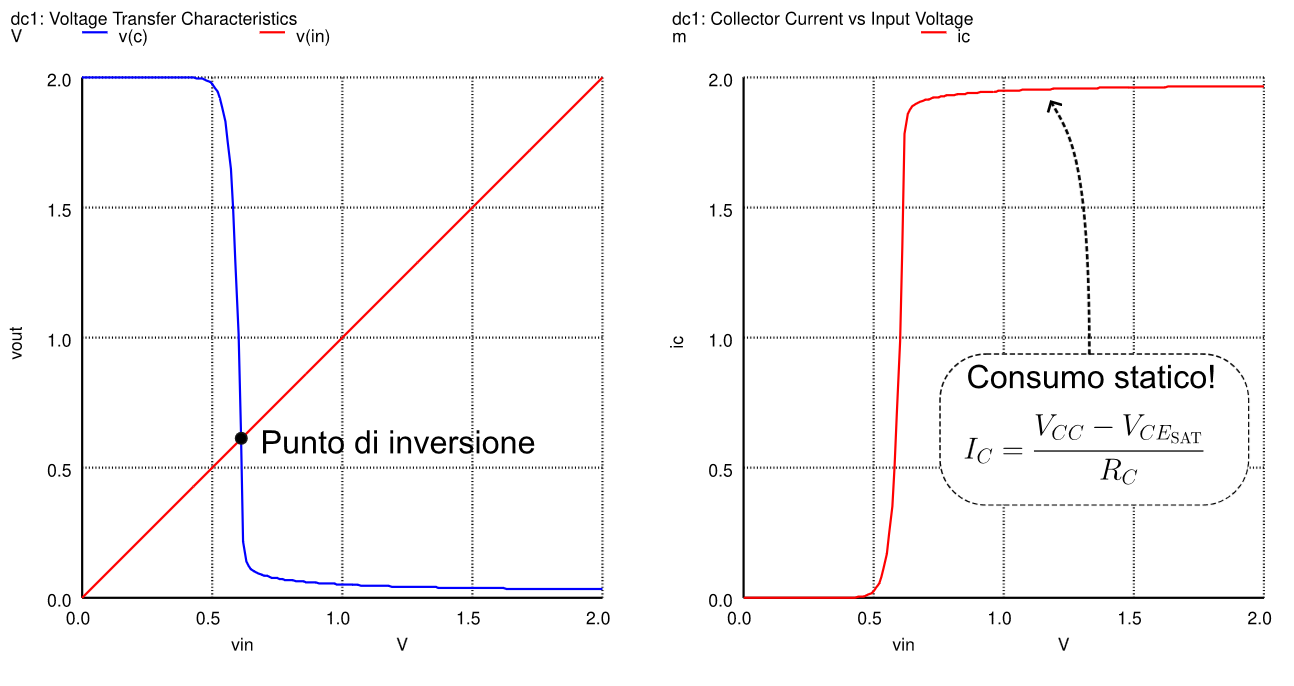
\includegraphics[scale=0.3]{../figures/bjt_invert_graph.png}
\end{center}

Ciò che notiamo è che per tensioni in ingresso basse, come abbiamo detto, otteniamo valori logici in uscita alti, e per tensioni di ingresso alte, otteniamo valori logici in uscita bassi. Questo è in sintonia con il funzionamento che ci aspettiamo dall'inverter. Notiamo anche che nella zona centrale abbiamo una decrescita della tensione $V_{out}$ (perché ci troviamo nella regione ZAD e ci stiamo spostando verso la saturazione), fino ad un punto (cosiddetto di \textit{inversione}) incontrato quando la $V_{in}$ incrocia la $V_{out}$.

Notiamo che questo design dell'inverter solleva uno dei punti critici che avevamo notato in 7.1.3: quando siamo nello stato $V_{in}$ alto (e quindi $V_{out}$ basso), stiamo consumando corrente a vuoto, cioè la corrente di colletore che avevamo considerato nella regione di saturazione:
$$
I_C = \frac{V_{CC} - V_{CE \, \mathrm{sat}}}{R_C}
$$
Questa caratteristica, che purtroppo è necessaria per avere il corretto funzionamento dell'inverter, porta ad un consumo di energia costante ogni volta che l'inverter è in inversione con segnale $V_{out}$ basso.

\subsection{Amplificazione coi BJT}
Vediamo, considerando sempre lo stesso circuito (presentato come un inverter) della sezione precedente, come un transistore BJT può comportarsi da \textit{amplificatore} di potenza per un dato segnale di ingresso.

Si ha infatti che l’inverter a carico resistivo si comporta come un amplificatore di tensione invertente se l’ingresso è polarizzato nella zona di transizione. Questo si ricava direttamente dal grafico della $V_{out}$ in funzione della $V_{in}$ riportato prima:

\begin{center}
	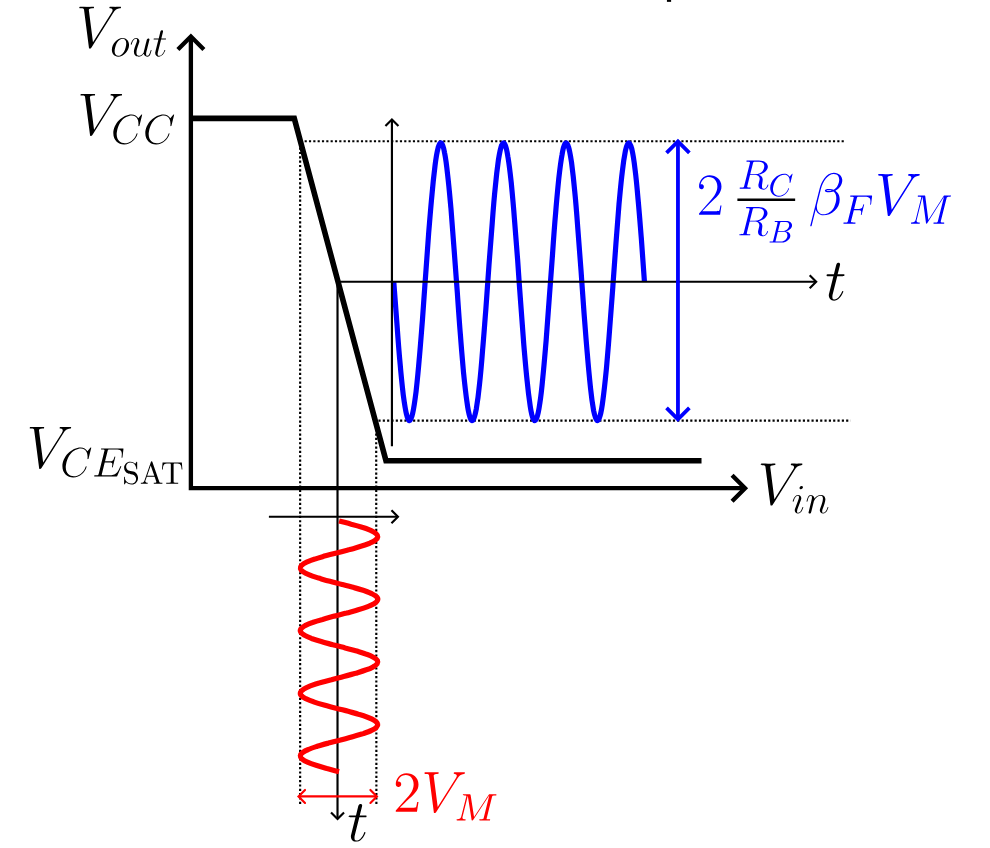
\includegraphics[scale=0.25]{../figures/bjt_invert_amp.png}
\end{center}

cioè introducendo alla $V_{in}$ un segnale ristretto alla regione che porta il transistore a lavorare in ZAD, che ricordiamo era:
$$
V_\gamma \leq V_{in} < V_{in \, \mathrm{sat}}
$$
si ottiene sulla $V_{out}$ lo stesso segnale, invertito, ed amplificato da $V_{CE \, \mathrm{sat}}$ a $V_{CC}$.
L'amplificazione di tensione sarà la seguente:
$$
A_V = - \beta_F \frac{R_C}{R_B}
$$
Notiamo che un difetto di questo circuito è che l’amplificazione può variare fortemente con i parametri del transistore e la temperatura. Per questo avremo bisogno di realizzare reti amplificatrici migliori.

\subsubsection{Rete a 4 resistori}
Abbiamo quindi detto che è necessario fissare una corrente continua costante di collettore o di emettitore che sia poco sensibile alle variazioni della temperatura e dei parametri del transistor.

Consideriamo allora la seguente rete (a 4 restistori):
\begin{center}
\begin{circuitikz}
	\draw
(0,0) node[ground]{} to[R=$R_2$] (0,3)
to[R=$R_1$] (0,6) node[vcc]{};

\draw (0,3) -- (2,3);

\draw (2,3) node[npn, anchor=B] (Q1) {};

\draw (Q1.C) to[R=$R_C$] ++(0,3) node[vcc]{};
\draw (Q1.E) to[R=$R_E$] ++(0,-3) node[ground]{};

\draw[->] (1.2,3.3) -- (1.8,3.3) node[midway, above]{$I_B$};
\draw[->] (Q1.C) ++(0.3,0.5) -- ++(0,-1) node[midway, right]{$I_C$};
\draw[->] (Q1.E) ++(0.3,0) -- ++(0,-.8) node[midway, right]{$I_E$};
\end{circuitikz}
\end{center}

Ciò che facciamo innanzitutto riportarci all'equivalente di Thevenin del partitore di tensione a sinistra, ricordando che:
$$
V_{BB} = \frac{R_2}{R_1 + R_2} V_{CC} \implies 
R_{B} = \frac{R_1 R_2}{R_1 + R_2}
$$

\begin{center}
\begin{circuitikz}
\draw
(8,0) node[ground]{} to[V=$V_{BB}$] (8,3)
to[R=$R_B$] (10,3);

\draw (10,3) node[npn, anchor=B] (Q2) {};

\draw (Q2.C) to[R=$R_C$] ++(0,3) node[vcc]{};
\draw (Q2.E) to[R=$R_E$] ++(0,-3) node[ground]{};

\draw[->] (9.4,3.3) -- (10,3.3) node[midway, above]{$I_B$};
\draw[->] (Q2.C) ++(0.3,0.5) -- ++(0,-1) node[midway, right]{$I_C$};
\draw[->] (Q2.E) ++(0.3,0) -- ++(0,-.8) node[midway, right]{$I_E$};
\end{circuitikz}
\end{center}

Quindi facciamo l'ipotesi di funzionamento in ZAD (che era la stessa ipotesi dell'amplificatore di prima), imponendo il modello ideale e quindi ricavando:
\[
	\begin{cases}
		V_{BB} = R_B I_B + V_\gamma + R_E I_E \\
		V_{CC} = R_C I_C + V_{CE} + R_E I_E \\
		I_C = \beta_F I_B \\
		I_E = I_C + I_B = (\beta_f + 1)I_B
	\end{cases}
\]

Risolvendo tale sistema si ottiene:
$$
I_E = (\beta_f + 1)I_B = \frac{ V_{BB} - V_\gamma }{ \frac{R_B}{\beta_F + 1} + R_E }
$$
che se:
$$
\begin{cases}
	V_{BB} >> V_\gamma \\
	R_E >> \frac{R_B}{\beta_F + 1}
\end{cases} \implies
I_E \approx I_C \approx \frac{V_{BB}}{R_E} 
$$
Cioè la corrente di emettitore e, quindi, quella di collettore, sono determinate dai componenti esterni collegati al transistore.

\end{document}
